\documentclass[final,t]{beamer}

% retrieved from
% http://www-i6.informatik.rwth-aachen.de/~dreuw/latexbeamerposter.php

% {{{ preamble

% Siebel poster printer paper width -- ANSI E: 34"x44"
% Fedex Office: 24"x36" or 36"x48"

\pgfmathsetmacro{\posterheight}{34*2.54}
\pgfmathsetmacro{\posterwidth}{22*2.54}

\usepackage[orientation=landscape,size=custom,width=\posterwidth,height=\posterheight,scale=1.18]{beamerposter}

\mode<presentation>
\usetheme{uiucposter}

% {{{ additional packages

\usepackage{lipsum}
\usepackage[utf8]{inputenc}
%\usepackage{times}
\usepackage{amsmath,amsthm, amssymb, latexsym}
\usepackage[T1]{fontenc}
\usepackage{lmodern}
\usepackage{exscale}
%\usepackage[lighttt]{lmodern}
%\boldmath
\usepackage{booktabs, array}
%\usepackage{rotating} %sideways environment
\usepackage[english]{babel}
\usepackage{wrapfig}
\usepackage[skins,listings]{tcolorbox}

\pgfdeclarelayer{foreground}
\pgfsetlayers{main,foreground}

% }}}

%\usepackage{svg}

% {{{ tikz

\usepackage{tikz}
\usetikzlibrary{calc}
\usetikzlibrary{positioning}
\usetikzlibrary{fadings}
\usetikzlibrary{chains}
\usetikzlibrary{scopes}
\usetikzlibrary{shadows}
\usetikzlibrary{arrows}
\usetikzlibrary{snakes}
\usetikzlibrary{shapes.misc}
\usetikzlibrary{shapes.symbols}
\usetikzlibrary{shapes.multipart}
\usetikzlibrary{fit}
\usetikzlibrary{shapes.arrows}
\usetikzlibrary{shapes.geometric}
\usetikzlibrary{shapes.callouts}
\usetikzlibrary{decorations.text}

% }}}

% {{{ box config

\tcbset{toplevelbox/.style={%
    enhanced,
    fuzzy shadow={5mm}{-5mm}{0mm}{1mm}{gray},
    colback=white,
    fonttitle=\bfseries,
    coltitle=white,
    colframe=uiucblue,
    boxsep=20pt,
    arc=10pt,
    top=0pt,
    boxrule=0pt,
    toptitle=-10pt,
    bottomtitle=-10pt,
    enlarge bottom by=1.25cm,
    titlerule=0pt,
  }
}

% }}}

% {{{ listing config

\tcbset{listing engine=listings}
\tcbset{listingbox/.style={%
    enhanced,
    %boxsep=-9pt,
    %left=15pt,
    arc=7pt,
    enlarge top by=4mm,
    %enlarge bottom by=1mm,
    boxrule=2pt,
  }
}

\definecolor{green}{RGB}{0, 180, 0}

\lstdefinestyle{custompython}{%
  %belowcaptionskip=1\baselineskip,
  breaklines=true,
  frame=none,
  xleftmargin=\parindent,
  language=Python,
  showstringspaces=false,
  basicstyle=\ttfamily,
  keywordstyle=\bfseries\color{uiucblue},
  commentstyle=\itshape\color{purple},
  identifierstyle=\color{black},
  stringstyle=\color{uiuclightblue},
  keywords=[2]{as,True,False},
  keywordstyle=[2]\bfseries\color{green!40!black},
  otherkeywords={>>>,...},
  keywordstyle=[3]\bfseries\color{blue},
  numbers=none,
  columns=flexible,
  rangebeginprefix=\>\>\>\ \#\ ,
  rangeendprefix=\>\>\>\ \#\ ,
  includerangemarker=false,
}

\newtcbinputlisting{\mylisting}[2][]{%
  listing file={#2},
  listingbox,
  listing only,
  listing options={style=custompython,linerange=#1},
}

% }}}

% Display a grid to help align images
%\beamertemplategridbackground[1cm]

% }}}


% {{{ front matter

\title{Mortar Spectral Element Method}
\author{Malachi Phillips \texttt{<malachi2@illinois.edu>}}
\institute{%
  Computer Science
  $\cdot$ University of Illinois
}
\date{May 8, 2019}

% }}}

\begin{document}
\begin{frame}[fragile]{}
  \begin{columns}[t]

    % {{{ left column

    \begin{column}{.45\linewidth}
      \begin{tcolorbox}[toplevelbox,adjusted title={Problem Statement}]
      Often in finite element methods, resolving a boundary layer requires
      the use of tighly packed elements throughout the mesh. In conforming
      elements, such an arrangement incurs the penalty of bad aspect ratio elements.
      The effect of pouring in additional conforming elements at the boundary layer
      further results in an undue number of elements, especially far away from the
      boundary layer itself. However, by relaxing the $H^1$ constraint of the
      conforming spectral element method (SEM), one may achieve greater flexibility
      in the spectral decomposition, allowing for $p$-adaptivity of elements near
      boundary layers. This is known as the mortar spectral element method (MSEM).
      \end{tcolorbox}

      \begin{tcolorbox}[toplevelbox,adjusted title=Approach]
      \begin{figure}
      \begin{center}
      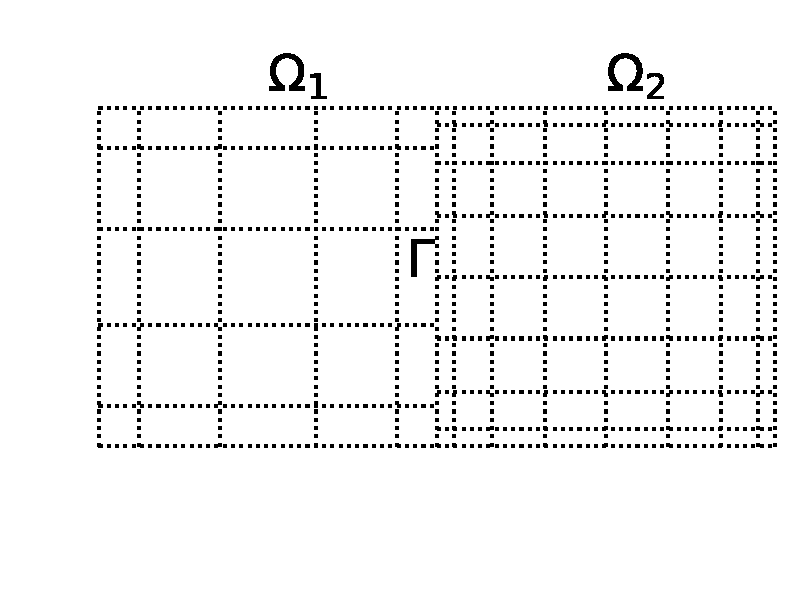
\includegraphics[
  width=\textwidth
]{omega1omega2}
\end{center}

\caption{\label{fig:domaindecomp} Example of a geometrically confroming domain decomposition, $N_1 = 5$ and $N_2 = 8$.}
      \end{figure}
\begin{enumerate}
\def\labelenumi{\arabic{enumi}.}
\item
  Divide \(\Omega\) into \(E\) nonoverlapping subdomains, such that
  \(\Omega=\bigcup_{e=1}^{E} \Omega ^e\).
\item
  Assign (non-unique) mortars to the surfaces between two different subdomains, assigning dependent and independent sides.
\item
  Across the interface, \(\Gamma\), between two elements \(i\) and
  \(j\), impose an \(L_2\) continuity requirement
  \(\int_{\Gamma}(u_i-u_j)\psi d\tau = 0\ \forall \psi \in \mathbb{P}_{N_i-2}(\Gamma)\).
\end{enumerate}

For the two subdomain case with \(\Omega_1\) being the independent side and \(\Omega_2\)
being the dependent side and $N_1 \le N_2$, the continuity requirement from (3) results
in a simple interpolation scheme:
\begin{equation}
\tilde{u}^2(s) = \tilde{u}^1(s) + \alpha L_{N_2}(s) + \beta L_{N_2-1}(s) \nonumber ,
\end{equation}
where the coefficients, $\alpha$, $\beta$, are expressed in terms of $\tilde{u_0}^2$ and
$\tilde{u}_{N_2}^2$. Imposing direct continuity on the vertices of $\Omega_1$ and $\Omega_2$,
this further simplifiers into a (variable-resolution) conforming case, which is considered here.

      \end{tcolorbox}

      \begin{tcolorbox}[toplevelbox,adjusted title= Test Cases]
      Solve in rectangular domain (\ref{fig:domaindecomp}) $[-2,2]\times[-1,1]$
      the following PDEs (homogeneous Dirichlet B.C. on $\partial\Omega$):
\begin{enumerate}
\item
$-\Delta u = f$
\item
$\dfrac{\partial u}{\partial t} + \boldsymbol{c} \cdot \nabla u = \nu \Delta u +f$, for $t\in[0,3]$.
\end{enumerate}
      Compare convergence rates against SEM ($E=1,2$)
      and a MSEM ($E=2$) of varying polynomial degree.
      \end{tcolorbox}
    \end{column}

    % }}}

    % {{{ right column

    \begin{column}{.45\linewidth}

      \begin{tcolorbox}[toplevelbox,adjusted title=Results]
      \begin{figure}
      \begin{center}
      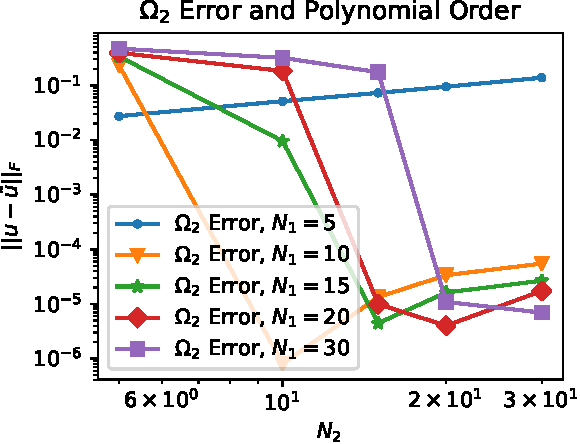
\includegraphics[
  width=\textwidth
]{errplot_pdf}
\end{center}

\caption{\label{fig:convplot} Error compared to true solution for Poisson's equation in $\Omega_2$.}
      \end{figure}
As shown in above figure, the MSEM converges for mixed polynomial orders. However, the error is minimized whenever the polynomial orders match.
      \begin{figure}
      \begin{center}
      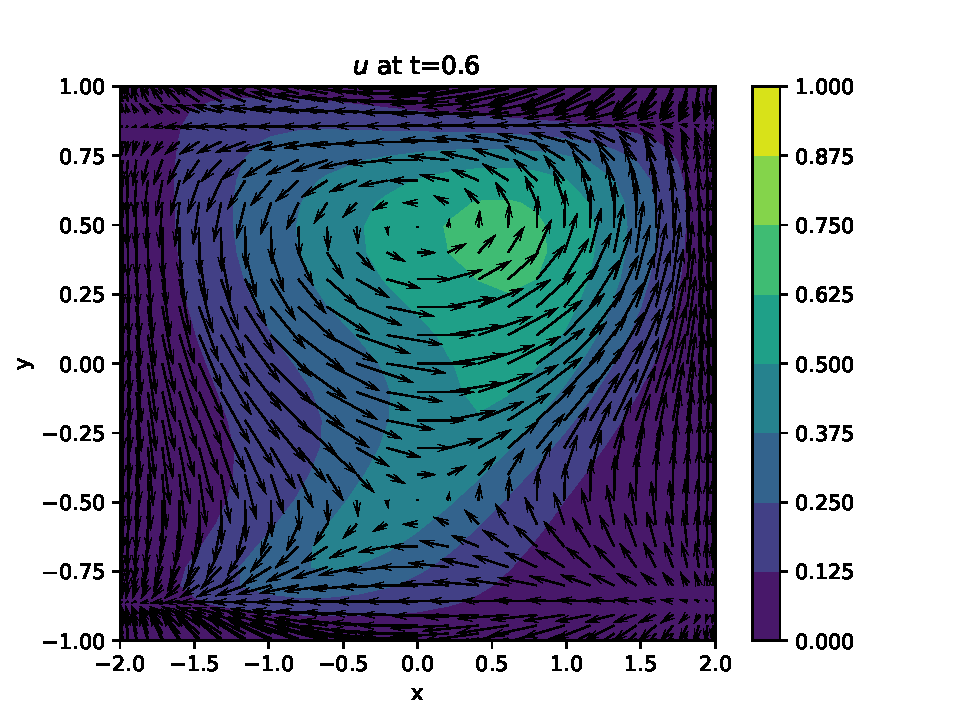
\includegraphics[
  width=\textwidth
]{../poster/conv_diff_single_elem_t_06}
\end{center}

\caption{\label{fig:convdiffplot} Convection-diffusion equation solution at $t=0.6 s$ for $E=1$ SEM, $p=30$.}
      \end{figure}
      
      \end{tcolorbox}

      \begin{tcolorbox}[toplevelbox,adjusted title=References]
      M. O. Deville, P. F. Fischer, and E. H. Mund, High-Order Methods for Incompressible Fluid Flow. Cambridge: Cambridge University Press, 2002.
      \end{tcolorbox}
      \begin{tcolorbox}[toplevelbox,adjusted title=GitHub]
      https://github.com/MalachiTimothyPhillips/MSE
      \end{tcolorbox}

    \end{column}

    % }}}

  \end{columns}
\end{frame}

\end{document}

% vim: foldmethod=marker
